\documentclass[handout]{beamer}

\usepackage{fontspec} 
% \usepackage{lsp-makros}
\useoutertheme{lsp}

\usepackage{lsptitle}

\def\two@digits#1{\ifnum#1<10 0\fi\number#1}
\def\mytoday{\two@digits{\number\day}.\two@digits{\number\month}.\number\year}


\usepackage{xspace,multicol}
\newcommand{\latex}{\LaTeX\xspace}
\usepackage{tikz}
\usetikzlibrary{positioning}


\newcounter{lastpagemainpart}
\footnotesep0pt
\renewcommand{\footnoterule}{}
\usefootnotetemplate{
  \noindent
  \insertfootnotemark\insertfootnotetext}

\let\beamerfn=\footnote
\renewcommand{\footnote}[1]{%
\let\oldfnsize=\footnotesize%
\let\footnotesize=\tiny%
\beamerfn<\thebeamerpauses->{#1}%
\let\footnotesize=\oldfnsize}


\date{2018-06-26, Radical Open Access, Coventry}

\usepackage{eurosym}  
 
\renewcommand{\centerline}[1]{\hfill#1\hfill\hfill\mbox{}}


\title{Outcompeting Gold}
\institute{Language Science Press}
\author[LangSci]{Sebastian Nordhoff}



\begin{document}
\lspbeamertitle

\section{Background}

\frame{
\frametitle{Linguistics}
\begin{itemize}
 \item   General linguistics a comparatively small field
 \item   25\,000 linguists worldwide
 \item   Books and articles
 \item Books at 100-200 EUR 
 \item Books sell <200 copies 
\end{itemize}
}


\frame{
\frametitle{Sebastian Nordhoff}
\begin{columns}
  \begin{column}{2cm}
   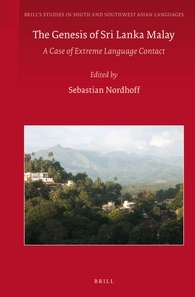
\includegraphics[width=2.5cm]{brill.jpg}
  \end{column}
  \begin{column}{7.5cm}
    \begin{itemize}
    \item PhD 2009, Universiteit van Amsterdam 
    \item \textit{A grammar of Upcountry Sri Lanka Malay}
    \item \textit{The genesis of Sri Lanka Malay} (Brill, 2012)
    \item \textit{Linked data in Linguistics} (with Christian Chiarcos and Sebastian Hellmann, Springer, 2012)
    \item \textit{Electronic grammaticography} (University of Hawai'i Press, 2012)
    \item Since 2014 coordinator for Language Science Press  
\end{itemize}
  \end{column}
\end{columns}

} 


\frame{
\frametitle{Language Science Press}
  \begin{itemize}
    \item monographs and edited volumes
    \item CC-BY
    \item  20 series, 160 editorial board members worldwide
    \item 70 published books, 350 expressions of interest
    \item up to >20.000 downloads per book
    \item open access, open source, open data
    \item consortial funding: 101 institutions worldwide for 1000 EUR/year via Knowledge Unlatched
    \item community-based publisher
    \begin{itemize}
     \item community proofreading 
     \item advisory board
     \item series editors meeting
    \end{itemize}
  \end{itemize}
}

\frame{
\frametitle{Language Science Press}
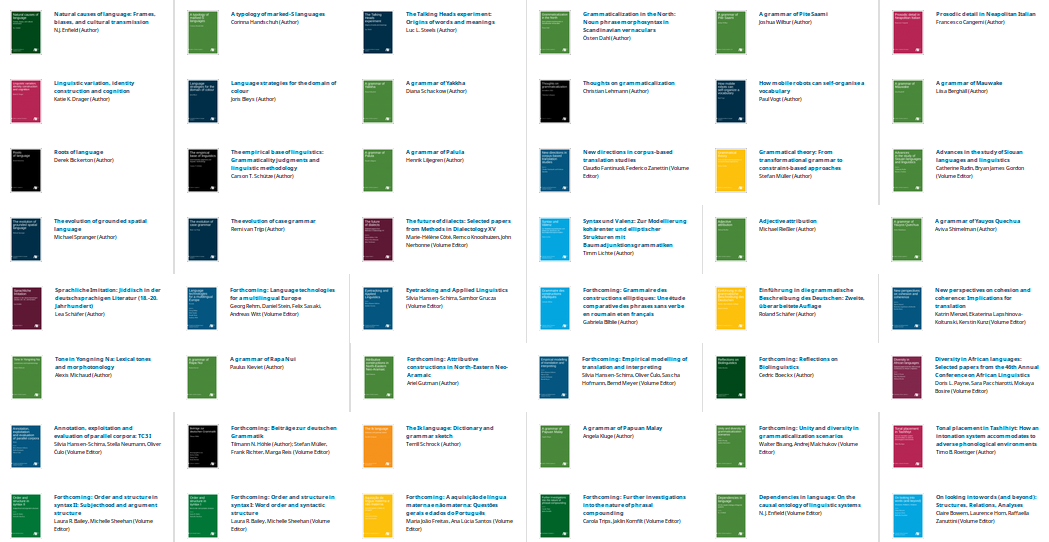
\includegraphics[width=\textwidth]{catalog.png} 

}

\section{Subscription model}
\frame{
\frametitle{\raggedright Flow of money in a reader-pays model}
\resizebox{7cm}{!}{
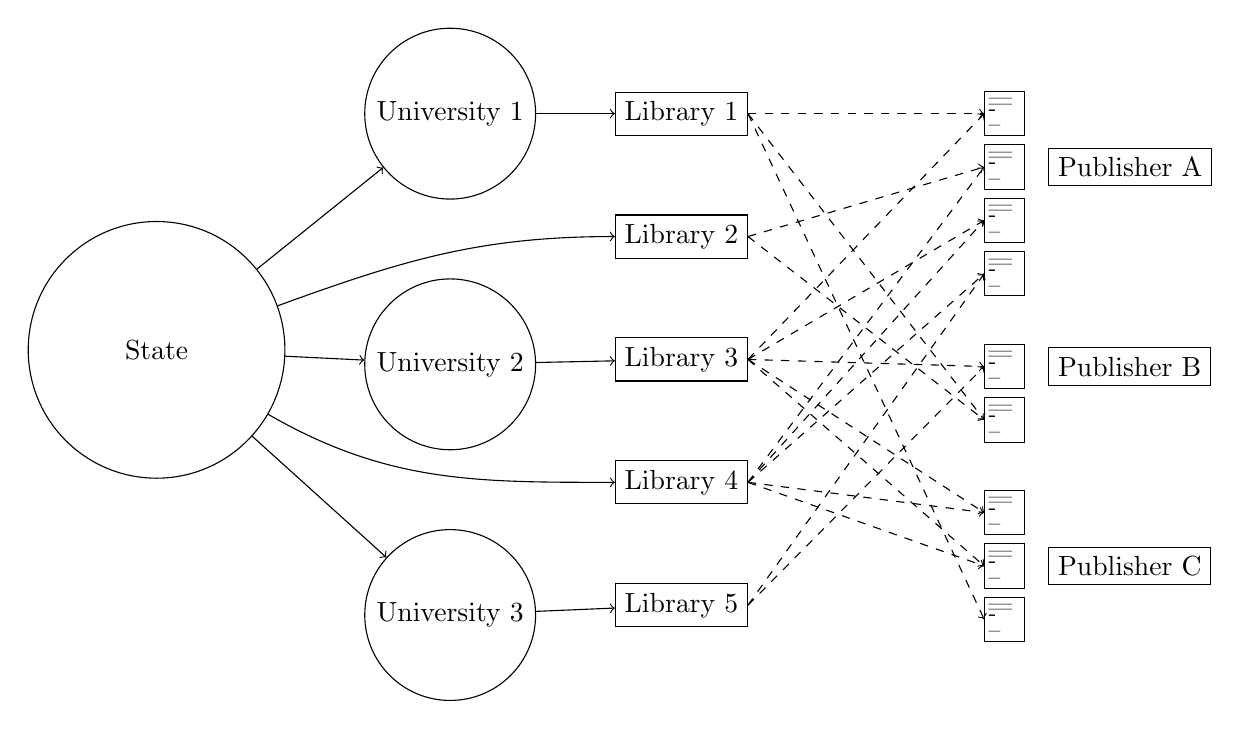
\begin{tikzpicture}
 \node[circle,draw,text width=3cm,align=center] (state) {State};
 \node[circle,draw] (university1) [right=of state,yshift=3cm] {University 1};
 \node[circle,draw] (university2) [below=of university1] {University 2};
 \node[circle,draw] (university3) [below=of university2] {University 3};
 \node[rectangle,draw] (library1)  [right=of university1]{Library 1};
 \node[rectangle,draw] (library2)  [below=of library1]{Library 2};
 \node[rectangle,draw] (library3)  [below=of library2]{Library 3};
 \node[rectangle,draw] (library4)  [below=of library3]{Library 4};
 \node[rectangle,draw] (library5)  [below=of library4]{Library 5};
 
 \node[rectangle,draw,text width=4mm, inner sep=0.5mm] (bookA1) [right=30mm of library1] {\footnotesize ---\\[-.9em]\footnotesize ---\\[-.9em]\footnotesize -\\[-.7em]--~};
 \node[rectangle,draw,text width=4mm, inner sep=0.5mm] (bookA2) [below=1mm of bookA1] {\footnotesize ---\\[-.9em]\footnotesize ---\\[-.9em]\footnotesize -\\[-.7em]--~};
 \node[rectangle,draw,text width=4mm, inner sep=0.5mm] (bookA3) [below=1mm of bookA2] {\footnotesize ---\\[-.9em]\footnotesize ---\\[-.9em]\footnotesize -\\[-.7em]--~};
 \node[rectangle,draw,text width=4mm, inner sep=0.5mm] (bookA4) [below=1mm of bookA3] {\footnotesize ---\\[-.9em]\footnotesize ---\\[-.9em]\footnotesize -\\[-.7em]--~};

 \node[rectangle,draw,text width=4mm, inner sep=0.5mm] (bookB1) [below=6mm of bookA4] {\footnotesize ---\\[-.9em]\footnotesize ---\\[-.9em]\footnotesize -\\[-.7em]--~};
 \node[rectangle,draw,text width=4mm, inner sep=0.5mm] (bookB2) [below=1mm of bookB1] {\footnotesize ---\\[-.9em]\footnotesize ---\\[-.9em]\footnotesize -\\[-.7em]--~};

 \node[rectangle,draw,text width=4mm, inner sep=0.5mm] (bookC1) [below=6mm of bookB2] {\footnotesize ---\\[-.9em]\footnotesize ---\\[-.9em]\footnotesize -\\[-.7em]--~};
 \node[rectangle,draw,text width=4mm, inner sep=0.5mm] (bookC2) [below=1mm of bookC1] {\footnotesize ---\\[-.9em]\footnotesize ---\\[-.9em]\footnotesize -\\[-.7em]--~};
 \node[rectangle,draw,text width=4mm, inner sep=0.5mm] (bookC3) [below=1mm of bookC2] {\footnotesize ---\\[-.9em]\footnotesize ---\\[-.9em]\footnotesize -\\[-.7em]--~};

 
 \node[rectangle,draw] (publisherA) [right=3mm of bookA2] {Publisher A};
 \node[rectangle,draw] (publisherB) [right=3mm of bookB1] {Publisher B};
 \node[rectangle,draw] (publisherC) [right=3mm of bookC2] {Publisher C};
%  \node[rectangle,draw] (staff)  [right=of publisher1] {Staff}; 
%  \node[rectangle,draw] (owners) [below=of staff] {Owners};
%  \node[rectangle,draw] (serviceproviders) [below=of owners] {Service providers};
%  \node[rectangle,draw] (etc) [below=of serviceproviders] {...};
 

% \path[draw] (box.north east) edge [->,transform canvas={yshift=-2mm}] (target.north west);

\path[draw] (state) edge [->] (university1);
\path[draw] (state) edge [->] (university2);
\path[draw] (state) edge [->] (university3);
\path[draw] (state) edge [->,out=20,in=180] (library2.west);
\path[draw] (state) edge [->,out=330,in=180] (library4.west);


\path[draw] (university1) edge [->] (library1);
\path[draw] (university2) edge [->] (library3);
\path[draw] (university3) edge [->] (library5);

\path[draw,dashed] (library1.east) edge [->] (bookA1.west);
\path[draw,dashed] (library1.east) edge [->] (bookB2.west);
\path[draw,dashed] (library1.east) edge [->] (bookC3.west);
\path[draw,dashed] (library2.east) edge [->] (bookA2.west);
\path[draw,dashed] (library2.east) edge [->] (bookB2.west);
\path[draw,dashed] (library3.east) edge [->] (bookA1.west);
\path[draw,dashed] (library3.east) edge [->] (bookA3.west);
\path[draw,dashed] (library3.east) edge [->] (bookB1.west);
\path[draw,dashed] (library3.east) edge [->] (bookC1.west);
\path[draw,dashed] (library3.east) edge [->] (bookC2.west);
\path[draw,dashed] (library4.east) edge [->] (bookA4.west);
\path[draw,dashed] (library4.east) edge [->] (bookA2.west);
\path[draw,dashed] (library4.east) edge [->] (bookA3.west);
\path[draw,dashed] (library4.east) edge [->] (bookC1.west);
\path[draw,dashed] (library4.east) edge [->] (bookC2.west);
\path[draw,dashed] (library5.east) edge [->] (bookA4.west);
\path[draw,dashed] (library5.east) edge [->] (bookB1.west);
\end{tikzpicture}
}
\begin{itemize}
 \item Every title is paid for by multiple institutions
 \item Unclear, how much money the publisher makes 
\end{itemize}
}
\section{Gold}

\frame{
\frametitle{\raggedright Flow of money in an author-pays model}
\resizebox{7cm}{!}{
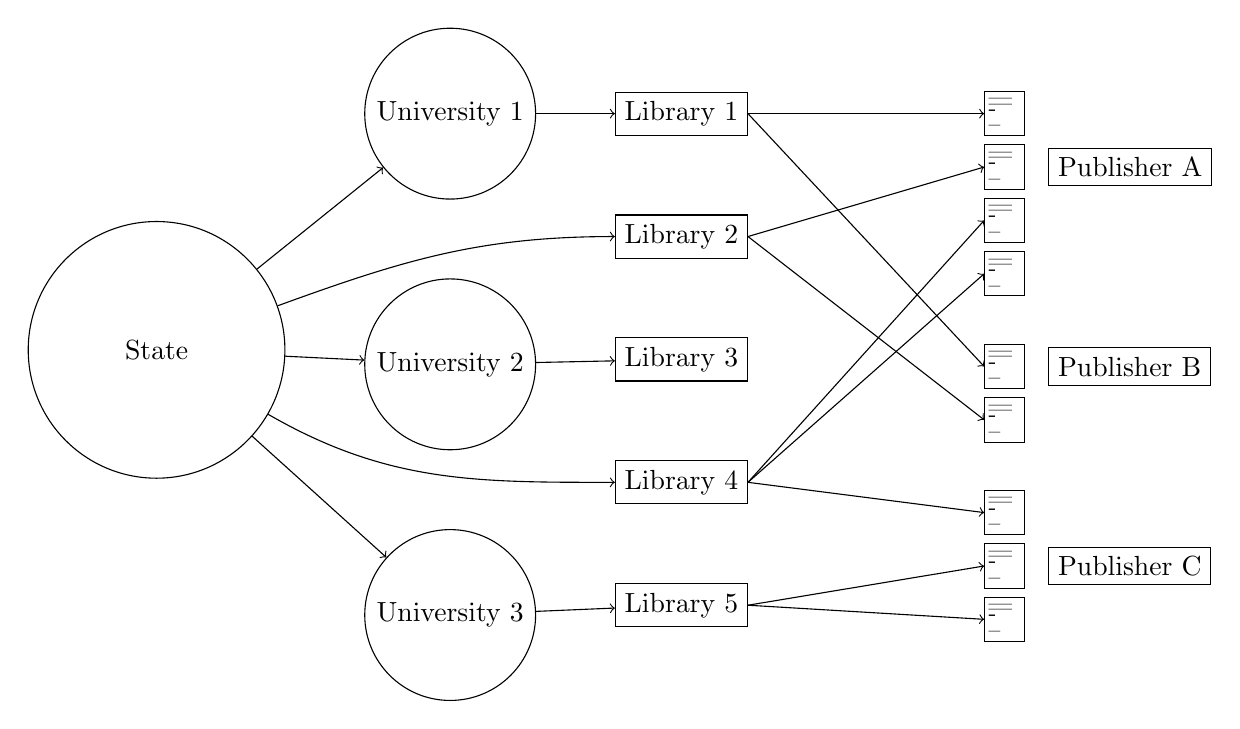
\begin{tikzpicture}
 \node[circle,draw,text width=3cm,align=center] (state) {State};
 \node[circle,draw] (university1) [right=of state,yshift=3cm] {University 1};
 \node[circle,draw] (university2) [below=of university1] {University 2};
 \node[circle,draw] (university3) [below=of university2] {University 3};
 \node[rectangle,draw] (library1)  [right=of university1]{Library 1};
 \node[rectangle,draw] (library2)  [below=of library1]{Library 2};
 \node[rectangle,draw] (library3)  [below=of library2]{Library 3};
 \node[rectangle,draw] (library4)  [below=of library3]{Library 4};
 \node[rectangle,draw] (library5)  [below=of library4]{Library 5};
 
 \node[rectangle,draw,text width=4mm, inner sep=0.5mm] (bookA1) [right=30mm of library1] {\footnotesize ---\\[-.9em]\footnotesize ---\\[-.9em]\footnotesize -\\[-.7em]--~};
 \node[rectangle,draw,text width=4mm, inner sep=0.5mm] (bookA2) [below=1mm of bookA1] {\footnotesize ---\\[-.9em]\footnotesize ---\\[-.9em]\footnotesize -\\[-.7em]--~};
 \node[rectangle,draw,text width=4mm, inner sep=0.5mm] (bookA3) [below=1mm of bookA2] {\footnotesize ---\\[-.9em]\footnotesize ---\\[-.9em]\footnotesize -\\[-.7em]--~};
 \node[rectangle,draw,text width=4mm, inner sep=0.5mm] (bookA4) [below=1mm of bookA3] {\footnotesize ---\\[-.9em]\footnotesize ---\\[-.9em]\footnotesize -\\[-.7em]--~};

 \node[rectangle,draw,text width=4mm, inner sep=0.5mm] (bookB1) [below=6mm of bookA4] {\footnotesize ---\\[-.9em]\footnotesize ---\\[-.9em]\footnotesize -\\[-.7em]--~};
 \node[rectangle,draw,text width=4mm, inner sep=0.5mm] (bookB2) [below=1mm of bookB1] {\footnotesize ---\\[-.9em]\footnotesize ---\\[-.9em]\footnotesize -\\[-.7em]--~};

 \node[rectangle,draw,text width=4mm, inner sep=0.5mm] (bookC1) [below=6mm of bookB2] {\footnotesize ---\\[-.9em]\footnotesize ---\\[-.9em]\footnotesize -\\[-.7em]--~};
 \node[rectangle,draw,text width=4mm, inner sep=0.5mm] (bookC2) [below=1mm of bookC1] {\footnotesize ---\\[-.9em]\footnotesize ---\\[-.9em]\footnotesize -\\[-.7em]--~};
 \node[rectangle,draw,text width=4mm, inner sep=0.5mm] (bookC3) [below=1mm of bookC2] {\footnotesize ---\\[-.9em]\footnotesize ---\\[-.9em]\footnotesize -\\[-.7em]--~};

 
 \node[rectangle,draw] (publisherA) [right=3mm of bookA2] {Publisher A};
 \node[rectangle,draw] (publisherB) [right=3mm of bookB1] {Publisher B};
 \node[rectangle,draw] (publisherC) [right=3mm of bookC2] {Publisher C};
%  \node[rectangle,draw] (staff)  [right=of publisher1] {Staff}; 
%  \node[rectangle,draw] (owners) [below=of staff] {Owners};
%  \node[rectangle,draw] (serviceproviders) [below=of owners] {Service providers};
%  \node[rectangle,draw] (etc) [below=of serviceproviders] {...};
 

% \path[draw] (box.north east) edge [->,transform canvas={yshift=-2mm}] (target.north west);

\path[draw] (state) edge [->] (university1);
\path[draw] (state) edge [->] (university2);
\path[draw] (state) edge [->] (university3);
\path[draw] (state) edge [->,out=20,in=180] (library2.west);
\path[draw] (state) edge [->,out=330,in=180] (library4.west);


\path[draw] (university1) edge [->] (library1);
\path[draw] (university2) edge [->] (library3);
\path[draw] (university3) edge [->] (library5);

\path[draw] (library1.east) edge [->] (bookA1.west);
\path[draw] (library1.east) edge [->] (bookB1.west);
\path[draw] (library2.east) edge [->] (bookA2.west);
\path[draw] (library2.east) edge [->] (bookB2.west);
\path[draw] (library4.east) edge [->] (bookA4.west);
\path[draw] (library4.east) edge [->] (bookA3.west);
\path[draw] (library4.east) edge [->] (bookC1.west);
\path[draw] (library5.east) edge [->] (bookC2.west);
\path[draw] (library5.east) edge [->] (bookC3.west);
\end{tikzpicture}
}
\begin{itemize}
 \item Every title is paid for by exactly one institution
 \item Revenue of publisher is absolutely clear and transparent
\end{itemize}
}

\subsection{Commodification}

\frame{
\frametitle{Commodification }
%   regalbild
\begin{itemize}
 \item buyer and seller are clearly identifiable in a Golden setup
 \item buyers will shop around 
 \item bang for the buck 
%  \item value for money
 \item monitoring: min, max, average, median 
 \item prediction: service providers for selecting the ``right'' journal. 
\end{itemize}
}



\subsection{Threats}
\frame{
\frametitle{The Golden Threat for books}
\begin{itemize}
 \item price tag
 \begin{itemize}
  \item easier to get 10 * 1000 EUR APCs than 1 * 10.000 EUR BPC
  \begin{itemize}
   \item or 100 * 100 with reader-pays
  \end{itemize}
  \end{itemize}
\item standardization
  \begin{itemize}
  \item ``A book costs 5000 EUR, period''
  \item once the vocabulary is established, ideas outside of that vocabulary become difficult to express
  \end{itemize}
\end{itemize}
}

  
\section{Competition}
\frame{
\frametitle{Competition in  Academia}
picture with anecdote
}

\section{Principles}
\frame{
\frametitle{\raggedright Principles for successful\newline collaborative publishing\newline  platforms}
\begin{itemize}
 \item attribution
 \item brands
 \item calculations
\end{itemize}
}


\frame{
\frametitle{Attribution}
\begin{columns}
  \begin{column}{5cm}
\begin{itemize}
 \item People want to belong 
 \item Recognition is a powerful incentive
 \item Division of labour 
 \begin{itemize}
  \item community-based effort
  \item senior academics do reviewing; junior academics do community proofreading
 \end{itemize}
\end{itemize}
  \end{column}
  \begin{column}{5cm}
    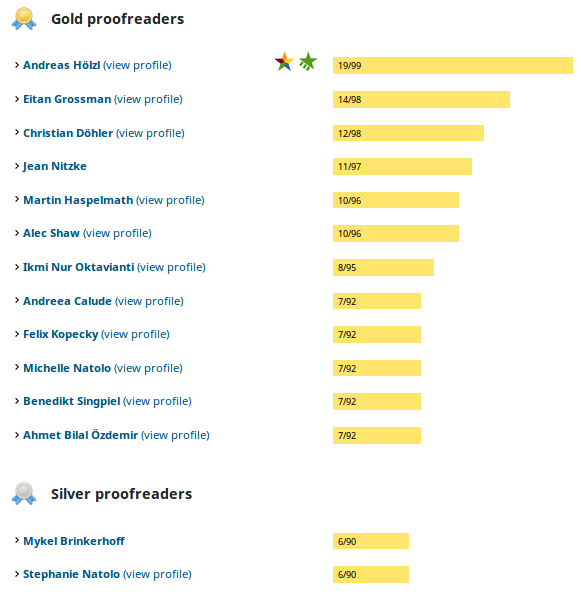
\includegraphics[width=5cm]{halloffame.png}
  \end{column}
\end{columns}
}


\frame{
\frametitle{Brands}
\begin{columns}
  \begin{column}{4cm}
\begin{itemize}
 \item Understand prestige
 \item You got 1 shot
 \item Protect your brand 
 \begin{itemize}
  \item Registration
  \item Mainly defensive, not offensive
 \end{itemize}
\end{itemize}
  \end{column}
  \begin{column}{6cm}
  
\includegraphics[width=6cm]{langsci_logo_nocolor.pdf}
  \end{column}
\end{columns}

}

\frame{
\frametitle{Calculations}
\begin{itemize}
 \item know your product. 
 \begin{itemize}
  \item What is it exactly that you provide? 
  \item Why is it valuable? 
  \item Valuable to whom? 
 \end{itemize}
  \item Know the resources required
  \begin{itemize}
   \item know-how
   \item technology 
   \item staff 
   \item funding
  \end{itemize}
  \item self-exploitation is not a business model!
  \item share your data!
\end{itemize}
}

\frame{
\frametitle{Neoliberal scum!}
% Gordon Gekko
The following concepts are related, but distinct: 	
\begin{itemize}
 \item Ownership of the means of production (capitalism)
 \item State intervention in the economy (neoliberalism)
 \item Business calculations (accountancy) 
 \item Standardization of products (commodification) 
 \item Competition/collaboration 
\end{itemize}
}

\section{Metallurgy}      
 
\frame{
\frametitle{OA metallurgy according to JS Caux}

\begin{columns}
  \begin{column}{7cm}
  \begin{itemize}
    \item \textbf{Gold [Au]} 	
    \begin{itemize}
     \item APC-based financing
    \end{itemize}
    \item \textbf{Platinum [Pt]} 	
    \begin{itemize}
     \item no charges for authors (APCs, submission charges or any other)
     \item funded through a consortial scheme or equivalent
    \end{itemize}
    \item \textbf{Palladium [Pd]} 
    \begin{itemize}
     \item purely not-for-profit public enterprise 
     \item none of the activities generate any profit
     \item all financial statements are publicly disclosed
    \end{itemize}
%     \bigskip
%     \pause 
%     \item Iron [Fe]	subscription-based financing, or pay-to-read
%     \item Lead [Pb] 	editorial and financial aspects are not hermetically decoupled
  \end{itemize}
  \end{column}
  \begin{column}{4cm}
    
\includegraphics[width=4cm]{jscaux.jpg}\vfill	
\footnotesize
\url{https://jscaux.org/blog/post/2017/09/20/noble-metals-noble-cause/}
  \end{column}  
\end{columns}
} 

\section{Full disclosure}

\frame{
\frametitle{OpenAire project:\\ Full disclosure}
\begin{tabular}{c|c}
 
\includegraphics[height=2cm]{cookbook.png} &   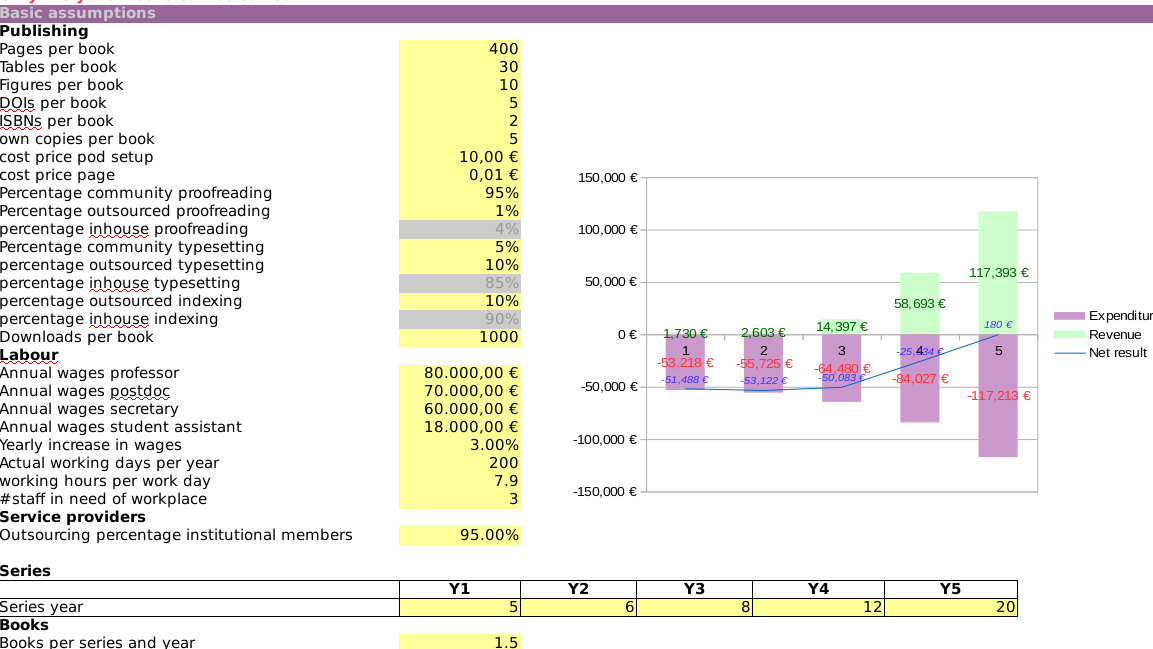
\includegraphics[height=2cm]{5y.png} \\  
 \hline\\
 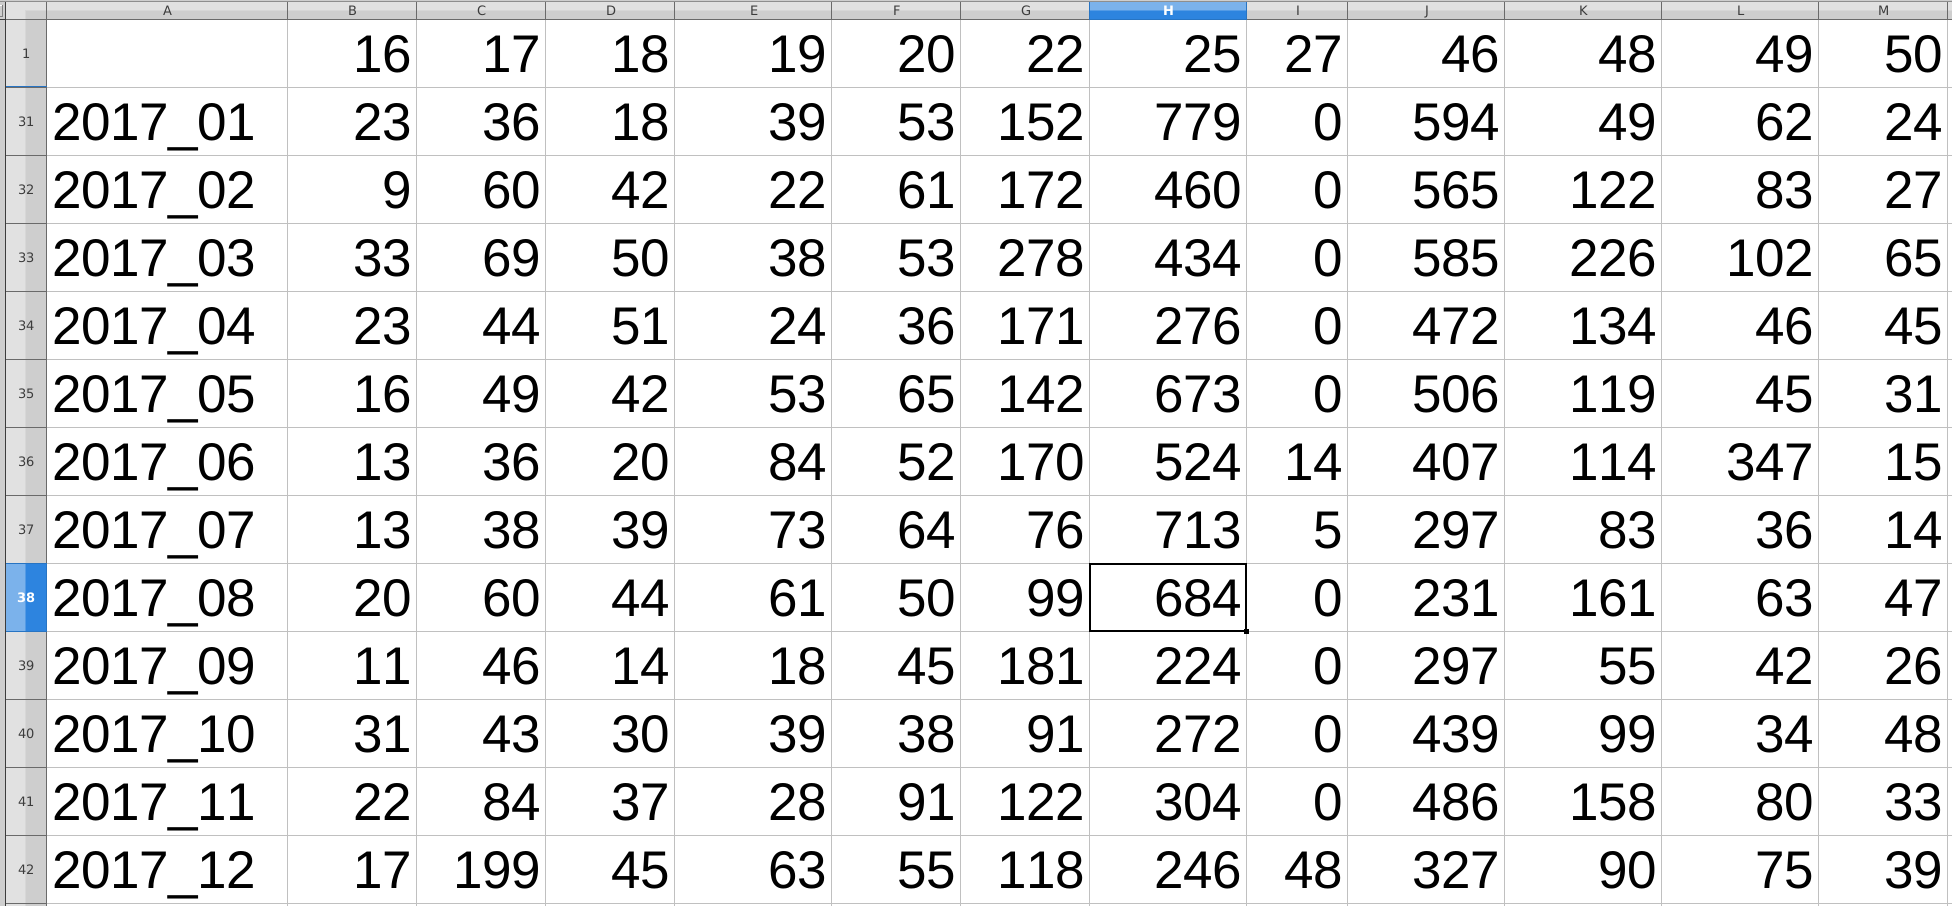
\includegraphics[height=2cm]{downloadfigures.png} &~\vspace*{13mm}~ 
\includegraphics[height=2cm]{businessmodel.png} 
\end{tabular}
\vspace*{-1cm}
\begin{itemize}
 \item Bottom line: LangSci books cost 3-4k€ total
 \item Various studies report costs of 10-35k€ per book for reader-pays models. 
\end{itemize}
}

\section{Conclusion}
\frame{
\frametitle{Wrapping up}
\begin{itemize}
 \item Publishers should watch their figures
 \item Collaborative publishers should disclose their figures
 \item Nice result: the figures actually show that collaboration outcompetes competition. 
\end{itemize}
}
  
%\setcounter{framenumber}{\thelastpagemainpart}
\end{document}